\documentclass{report}
\usepackage[utf8]{inputenc}
\usepackage[T1]{fontenc}
\usepackage{natbib}
%\usepackage{gfsartemisia-euler}
\usepackage{fourier}
\usepackage[normalem]{ulem} 
%\usepackage{fontspec}
%\setromanfont{Gulliver}
%\setsansseriffont{Tahoma}

\usepackage[margin=1in]{geometry}
\usepackage{graphicx}
\usepackage{xcolor}
\usepackage{amsmath}
\usepackage[outdir=./images/]{epstopdf}
\usepackage[inline]{enumitem}
\newlist{listahorizontal}{enumerate*}{1}
\setlist[listahorizontal]{label=(\alph*)}

\usepackage{setspace}


\title{Smart usage of context information for the analysis, design, and generation of power-aware policies for mobile sensing apps\\[0.2cm]\small\emph{Technical Report}}

\author{Rafael Pérez Torres\\\small Doctorate Seminar}
\date{}


\begin{document}
\maketitle

\begin{abstract}
Mobile devices, in any of their presentations like smartphones, tables, wearables, have been adopted massively by people around the world.
The features included in these devices, like sensing capabilities, computing, storage, and communication facilities have provided a fast path for the creation of mobile apps for general and specific purposes, like entertainment or productivity.
The popularity of these apps have promoted smart devices to ideal partners for every day activities.

Thanks to the communication and sensing capabilities of smart devices, they become aware of their environment and allow to detect and understand information about user's context.
When user's context is employed, it is possible to enhance the information delivered to the user and provide a wider range of apps. Such apps, known as mobile sensing apps, are aware of changes in context and location, and are able to react in proper ways.

However, the usage of sensors has an inherent impact on the device battery, specially when long continuous sensing is required by the mobile app.
This work aims to understand user's context and leverage it to make a smarter usage of sensors through the introduction of energy-aware policies.
These policies can be employed to re-adapt the duty cycle of sensors depending on mobile app requirements and patterns detected from sensor data.
\end{abstract}

\setstretch{1.2}

\chapter*{Background and motivation}
% Decir que los dispositivos están presentes en todos lados%
Mobile devices are virtually everywhere.
From sophisticated smartphones and tablets to wearable non-invasive devices, mobility is the law.
According to the Ericsson Mobile Report \citep{Ericson2014} there were 1,900 millions of smartphone subscriptions and 300 millions of mobile PCs, tablets and mobile routers subscriptions in the 2013.
It is expected that by the end of 2019 there will be 5,600 millions and 700 millions of subscriptions, respectively.

% Decir que los dispositivos son capaces de comunicarse entre ellos mismos %
The high acceptance degree of smart devices has been achieved because of their Internet-enabled features in addition to the increasing storage and computing capabilities they offer.
Because of this, users employ smart devices as partners in every day activities.
Phone tasks, emailing, gaming, media playing, and web surfing are activities performed through mobile devices anywhere, anytime.
Moreover, smart devices are becoming able to interact with other devices leveraging short range wireless infrastructure like BT \footnote{BT, bluetooth.} and the recent NFC \footnote{NFC, Near Field Communication.}.

% Decir que gracias a sus capacidades de sensado pueden crearse aplicaciones sensibles a la ubicación y sensibles al contexto %
In addition to storage, computation, and wireless communication capabilities, mobile devices are shipped with a wide range of sensors that are employed to enhance the interaction with user.
Thanks to sensors, a mobile device is able to detect the level of light, sound, acceleration, orientation and even its location at any given moment.
By employing these facilities, mobile devices become \emph{omni-sensors} \citep{Perez-Torres2012} of user environment enabling the development of context aware mobile apps.

% Decir lo que es el contexto %
Although there is no a established definition of context, it can be understood as the set of environmental states and settings that either determines an application’s behavior or in which an application event occurs and is interesting to the user \citep{Chen2000}.
% Tell what sensors (apart from GPS) are emplyed by Mobile sensing apps
Typical examples of context in mobile devices are changes in accelerometers, gyroscopes, microphone, luminosity sensor, and more.

% Decir lo que es una aplicación sensible al contexto %
A context aware app is that which can detect changes in any context source of information and adapt its behavior depending on these changes.
Examples of apps that react to context are those that allow to change the display orientation according to the position of phone, control a videogame, adapt the screen brightness, detect user activity like running, walking or lying in bed, etcetera.


% Decir lo que es una aplicación sensible a la ubicación %
An important subset of context aware apps is conformed by location aware apps.
These apps can perceive changes in the location of the device and adapt its behavior depending on these changes.
The employed technology to obtain the location data can vary from mobile network cell, to wireless networks mechanisms and GPS \footnote{GPS, Global Positioning System.} infrastructure, in increasing order of precision.
% Tell generic examples of these applications
Typical examples of these applications include the tracking of people or automobiles \citep{Yuan2011}, detection of bottlenecks in traffic \citep{Thiagarajan2009} and sports tracking \citep{Lykke}.


% Tell context and location aware mobile apps are mobile sensing apps also
Location and context aware mobile apps share the characteristic of accessing sensors to obtain their \emph{awareness} and react accordingly.
From the hardware usage perspective, these apps have been categorized as \textbf{mobile sensing apps} and are a current trend in the mobile computing research area.
A mobile sensing app is such that relies its behavior completely on data collected from sensors and typically access them over long periods of time.

% Mention that MSA are helping to get the universal adoption of smart phone by society
Mobile sensing apps open a new way for the use of mobile devices and marks another step towards their universal adoption by society.
Such adoption has the implicit objective of leveraging even more their capabilities for closing the loop and employing them as the key to perform or improve the execution of any task.

% Mention that smart devices are producing a world where all people is connected
Smart devices are evolving the communication among society and are producing a world where most of humans are connected with each other.
% Tell that the smartphone is the user's identifier
Indeed, the smartphone is becoming an item that identifies and acts as a virtual agent of the user.
In this way, mobile devices represents a direct channel to establish communication with users and collect first-hand information about them.

% Tell that the globally connected idea has been also seen in industry by
This scenario of world globally connected entities has also been spotted in industry.
% ... enhancing real world items...
Industries have been able to keep the tracking of articles in supply chains, perform shipping and logistic tasks and many other activities by enhancing real world items with processing, computing, and communication capabilities and employing special techniques for their identification, like as RFID\footnote{Radio Frequency Identification.}.
% ... called smart objects that can get a M2M communication.
Such enhanced real world items are called \emph{smart objects} and when connected with other smart objects are capable of performing a \textbf{Machine to Machine (M2M)} communication \citep{Galetic2011}.

% Mention the goal of M2M
The final goal of the M2M communication is to go beyond the industry and connect every object of real world.
This communication can be performed in any direction (from real world item A to real world item B or vice-versa) in order to request data from objects or to instruct objects to react in specific ways.

% Mention that there is an analogy between the smart objects (m2m) and smart phone (mobile sensing apps)
Smart devices, like the smartphone, and smart objects share several characteristics, for example both have communication, storage and processing capabilities, both can be context aware by employing sensors, but at the end the set of tasks that can be done by them represents their difference.
% Mention the difference between smart objects and smart phones
Smartphone are entities with general purpose usage while smart objects are specific purpose only.
For instance, an smartphone can run several apps simultaneously that refer to entertainment or productivity tasks, but a enhanced blender will always be tied to its basic tasks.

As mentioned before, smart devices like the smartphone can be employed to identify users, just in the same way that RFID techniques are employed to identify smart objects.
Because smart objects and people can be identified, it is possible to construct a new global system that allows the communication among virtually any entity of real world.
State of art research abstracts these entities --- smart objects and smartphones ---, as \emph{things} and calls \textbf{The Internet of Thing (IoT)} to the system that connects them globally.

A definition of the IoT given in \citep{Sundmaeker2010} states that:

\begin{quotation}
The Internet of Things allows people and things to be connected \textbf{A}nytime, \textbf{A}nyplace, with \textbf{A}nything and \textbf{A}nyone, ideally using \textbf{A}ny path/network and \textbf{A}ny service.
\end{quotation}

The IoT is the next step in the evolution of current Internet.
As such, it will allow any object to become aware of its context, in terms of the physical environment and even its role in high level human tasks.
The final purpose is to make objects participants of business logic processes, not only sensors dispersed along a geographic area.
Because of this, devices will have a smarter behavior and interact with other devices without direct human participation.

However, IoT considers that humans can have a special and non distracting participation in some activities.
For instance, when a user arrives home, lights and a/c infrastructure should be turned on.
This implicit participation can be achieved by leveraging the smartphone as the virtual agent of people.
Hence, the smartphone can be employed as the key for triggering a very broad set of applications and systems.

% Decir que la energía es un factor que limita el uso de los dispositivos móviles %
The increasing use of mobile sensing apps is an instance of the convergence of mobile computing systems into the IoT, which will provide unlimited possibilities in the development of applications and scientific research opportunities.

However, despite all of the benefits that these systems would bring, there is an open issue when employing the mobile devices for such kind of tasks.
The problem is that advances in battery research are not at the same pace than those related to embedded sensors, computing, storage, and communication facilities \citep{Kjaergaard2012}.

Furthermore, this issue is likely to persist because of the mobility features of smart devices that require a small and lightweight battery in order to make the device truly portable.
The battery of any mobile device is a limited source of energy, which eventually will be drained because of sensors and other embedded electronics usage.
Because of such situation the time and diversity of tasks a device can be used for remains limited.

% Decir que el uso de la energía debe ser minimizado / maximizar la duración de la batería %
Therefore, it is mandatory for any mobile application development to consider the energy constraint and implement mechanisms or strategies to optimize battery duration, specially when accessing sensors in a continuous way over long periods of time.





\section{Problem statement}
% Mention that sensors allow killer apps ...
Sensors embedded in mobile devices allow developers to create location and context aware mobile apps with rich user content and smart behavior.
Indeed, this set of apps have created a new area of research called \textbf{mobile phone sensing} \citep{Lane2010}.

% Mention that sensors might be data-stream sensors
Some of these sensors deliver data streams in their readings.
% Mention what is a data-stream from our perspective
A data stream can be considered as a continuous and uninterrupted sequence of data whose elements can be processed and interpreted in an independent way.
% Mention a small set of examples of data stream based sensors
GPS, accelerometers, gyroscope and microphone are data stream sensors whereas a camera is not.

% ... but their usage has an implicit energy consumption
Despite all the benefits obtained by accessing sensors, it is also clear that it carries the implicit drawback of energy consumption.
For instance, in a common modern smartphone the highest energy consumer sensor and wireless communication interface are the GPS receiver and WiFi, respectively \citep{Kjaergaard2012}.
A mobile app employing frequently any of both elements is likely to impact heavily on the mobile device's battery performance.


% % Mention that in fact there are some apps which uses heavily obtaining user location via GPS
% Location aware mobile apps can be classified depending on their running time and power consumption, as seen in Figure \vref{fig:lsb-classification} (defined in \citep{Kjaergaard2012}).
% From that figure, it can be identified a type of mobile apps --- labeled as power minimized services --- whose requirements include obtaining user's location in a continue way over long periods of time.

% Mention that MSA access heavily to sensors.
Typically, mobile sensing apps access sensors in a continuous way over long periods of time.
For instance, a mobile sensing app may require to record a sound sample of 30 seconds length every 30 minutes as long as the app is running, or in other words permanently.
Applications like these have a high energy consumption due to task duration and the overhead generated by turning on and off the sensors.
This may lead to a quick battery drain that prevents smart device usage for other tasks.
% Mention what is the situation of the energy, Why is it 'very' important?
Mobile platforms must consider the energy as a scarce, shared and competed resource \citep{Perez-Torres2012}.

% Mention that current processors were not designed for performing sensor data analysis.
In addition, it must be noted that processors of current smart devices were designed to manage the heavy interaction with the user and the execution of mobile apps.
A continuous sensor reading is out of their current objectives, so there is a waste of energy when the processor is active only for reading data from sensors \citep{Priyantha2011}.
For example, a mobile app accessing the GPS in an uninterrupted way can drain the battery of a Samsung Galaxy S II smartphone in just 13 hours \citep{Perez-Torres2012}.

% \begin{figure}
% \centering
% 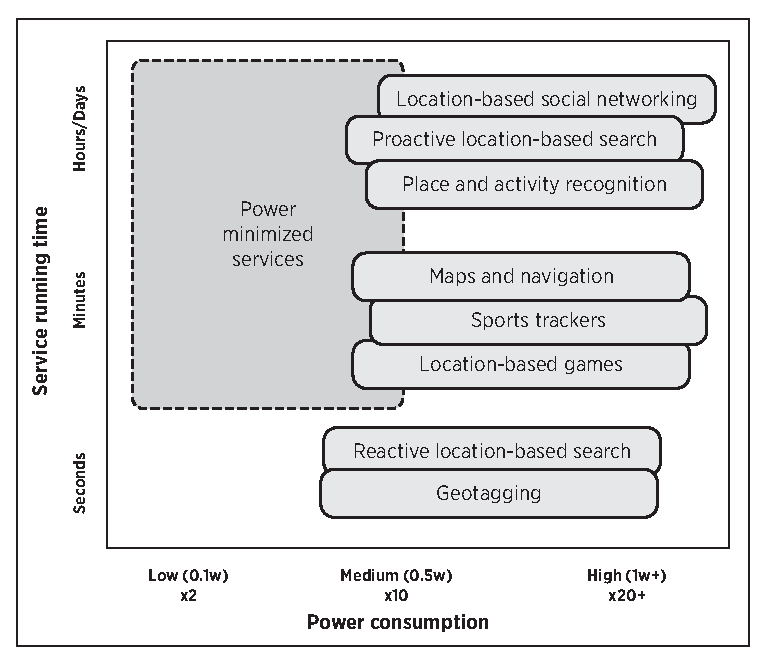
\includegraphics[scale=0.7]{lsb-classification}
% \caption[Location aware mobile apps classification by \protect\citep{Kjaergaard2012}]{Classification of location aware mobile apps based on its power consumption and running time, proposed by \protect\citep{Kjaergaard2012}.}
% \label{fig:lsb-classification}
% \end{figure}

% Mention the situation of current mobile apps
Current mobile platforms do not include out of the box mechanisms to perform periodical readings from sensors.
% Mention that API's of manufacturers always forget the business logic of the apps.
% This is understandable, API makers can not adapt to ALL particular requirements of mobile apps.
API's \footnote{API refers to Application Programming Interface, which is a library with a set of methods that performs logical related tasks. This library is available to programmers for software construction.} offered by manufacturers only accomplish generic tasks like turning on -- off sensors and reading data from them, but ignore app's business logic.
This means that mobile app requirements (like the precision in the sensor data collection), mobile device constraints (like the current level of battery), and threshold values for performing a smart sensor usage (for example, the lowest battery level for avoiding a permanent sensor usage) are always ignored by the mobile OS\footnote{Mobile OS, Mobile Operating System.} layers.

% Mention that there is a lack of a killer mechanism to perform operations like the ones described.
Therefore, there is the need of a specialized framework that considers previous elements and allows to generate smart policies for sensors usage when performing continuous readings.
A policy is a high level concept that defines the usage that sensors should observe in order to keep low energy consumption and accomplish mobile app requirements.
% The killer mechanism should be smart! The smartness will be obtained by identifying something in the sensor data, aka a pattern.
The \emph{smartness} of policies is achieved by leveraging the user's context obtained from data delivered by sensors.

% Mention that raw data is used to detect a pattern by the pattern identifier
At low level, the user's context can be identified by employing a \emph{pattern identifier} mechanism that is fed by raw data collected by sensors.
This pattern can represent for example a user mobility pattern which is helpful when generating the policy for accessing the GPS;
if the user mobility pattern describes motion of user at high speed, then the policy to be generated should instruct GPS readings more frequently than if user is moving at low speed.

% Mention that the pattern is employed by the policy generator to generate a smart policy
Hence, the pattern becomes a descriptor of user's context, and can be the input for a \emph{policy generator} mechanism that generates the policy that adapt the sensor usage, reduce the energy consumption and achieve mobile app objectives.

% Mention the importance of the hints.
An important aspect of these smart policies is the fact that their generation implies the specification of energy and precision hints.
These hints are necessary because the usage of sensors can be improved only when the mobile app specifies the level of precision required.
Such precision level dictates the granularity in the tracking of user activity.
However, the finer the granularity level of tracking, the higher the energy consumption due to sensor usage.
Then there is a trade-off between the precision and the energy consumption of mobile apps.

The proposed work aims the creation of needed mechanisms for the policies generation, and their implementation using the the GPS receiver and mobility patterns as proof of concept elements.

\subsection{Formal problem statement}
The problematic detected can be achieved by dividing it into two main problems, the pattern identification and the policy generation.
The pattern identification problem refers to the detection of a pattern in the data delivered by sensors.
This pattern helps to obtain information about user's context which is helpful to add smartness to the policy generation process.

On the other hand, the policy generation problem is related to the definition of a new duty cycle for accessing sensors.
This new duty cycle should reduce energy consumption and at the same time address the mobile app requirements.
\subsubsection{Pattern identification}

Given a set $V = \left\{v_{1}, v_{2}, \dotsc, v_{n}\right\}$ of data values read from sensor $S$ in the time interval $T  \in [t_{1}, t_{2}]$, find the behavior pattern $Pattern_{S}$ that represents the activity of user.

\begin{equation}
\text{PatternIdentifier}( V ) \longrightarrow{} \text{Pattern}_{S} \in \text{\textbf{Patterns}}
\end{equation}

Where $\text{\textbf{Patterns}}$ is a set of patterns that represent an interesting state in the user activity.
For instance, considering mobility data obtained from the GPS receiver, the set $\left\{\text{no\_movement}, \text{walking}, \text{running}, \text{vehicle\_transportation}\right\}$ can represent these interesting states.
The set of patterns is to be defined and conforms a step in the methodology.

\subsubsection{Policy generation}

Given the detected pattern $Pattern_{S}$ in data from sensor $S$, parameters for assigning weight to energy $eh$ and precision $ph$, and physical constraints status $pc$ of a mobile device, find a policy to adapt the duty cycle of sensors.

\begin{equation}
  PolicyGeneration( Pattern_{S}, eh, ph, pc ) \longrightarrow{} DutyCycle_{S}
\end{equation}

The policy will be generated considering the trade-off between energy and precision parameters that are specified by the mobile app, since both factors have an implicit impact on each other.

\subsection{Hypothesis}

Smart policies produced through context information built from sensors data can be employed to reduce the energy consumption in a mobile device when performing continuous sensor readings.

\subsection{Objectives}
Next are the objectives of the current research proposal.

\subsubsection{Main}

\emph{\sout{Reduce energy consumption when performing continuous sensor readings in mobile devices by making use of context information.}}

To reduce energy consumption in the mobile sensing apps, which perform continuous sensor readings, through power-aware policies generated from context information obtained from sensors data.
\subsubsection{Particulars}

\begin{itemize}
  \item \emph{\sout{Identify behavior patterns which can provide meaningful context information from raw data collected by sensors.}}
  \item To identify mobility patterns from context information obtained from an inertial sensor (accelerometer) and location providers (GPS, WPS).
  \item \emph{\sout{Generate smart policies for sensor usage from context information, mobile app requirements and mobile device constraints.}}
  \item To generate policies for a smart sensors' usage from mobility patterns, mobile app's accuracy and energy requirements, and status of mobile device's constraints. 
  \item {\color{blue} To ease the development of mobile sensing applications that require user location tracking, i.e., LBS, by means of a middleware that isolates the complexity of sensors' access and the associated efficient energy management.}
\end{itemize}


\section{Contributions}
This thesis work aims to produce the next contributions:
\begin{itemize}
  \item A mechanism for detecting mobility patterns from the data read by sensors of mobile devices (especifically GPS and accelerometer).
  \item A mechanism for generating policies for accessing sensors.
  Such mechanism employs application requirements (energy and precision hints), level of mobile device constraints, and user's context information (using the pattern detected by previous mechanism).
  The produced policies will allow to perform a smarter usage of smartphone's sensing infrastructure in continuous sensor readings, reducing the energy consumption.
  \item A middleware that implements the previously described mechanisms, easing the development of mobile sensing applications.
\end{itemize}


\bibliographystyle{unsrtnat}

\bibliography{../../../resources/references/bibliography}


\end{document}
